%       10        20        30        40        50        60       70        80        90        100
%234567890123456789012345678901234567890123456789012345678901234567890123456789012345678901234567890

\documentclass[dvipsnames,12pt]{article} % \documentclass{article}
\usepackage[utf8]{inputenc}

%%%%%%%%%%%%%%%%%%%%%%%%%%%%%%%%%%%%%%%%%%%%%%%%%%%%%%%%%%%%%%%%%%%%%%%%%%%%%%%%%%%%%%%%%%%%%%%%%%%%
%%%%%%%%%%%%%%%%%%%%%%%%%%%%%%  2024 WQ MATH 167 FPP REPORT TEMPLATE %%%%%%%%%%%%%%%%%%%%%%%%%%%%%%%
%%%%%%%%%%%%%%%%%%%%%%%%%%%%%%%%%%%%%%%%%%%%%%%%%%%%%%%%%%%%%%%%%%%%%%%%%%%%%%%%%%%%%%%%%%%%%%%%%%%%

% UNTIL SQ 2016 THIS WAS PROBLEM ?? IN HW 08

% MATH 167
% FALL QUARTER 2024
% 184 YOUNG HALL
%
%   Tue Mar 12 11:30:36 AM PDT 2024
%
%     REVISION HISTORY:
%
%       REVISION 1.00
%
%         Revision 1.00: Tue Mar 12 11:30:36 AM PDT 2024
%         Revision 1.01: Tue Mar 12 07:52:05 PM PDT 2024
%         Revision 1.02:
%         Revision 1.03:
%         Revision 1.04:
%         Revision 1.05:

%%%%%%%%%%%%%%%%%%%%%%%%%%%%%%%%%%%%%% SET UP PAGE PARAMETERS %%%%%%%%%%%%%%%%%%%%%%%%%%%%%%%%%%%%%%

% EGP's preferred page style for notes, homework assignments, exams, etc.

% Margins, paragraph indents, space between paragraphs if any, etc. Good references
% include page 85 of "The LaTeX Companion" by Frank Mittelbach and Michel Goossens and
% page 260 of "Math Into LaTeX" by George Gratzer.

% Enlarge the width and height of the printed page

\setlength{\textwidth }{08.00 in} % EGP's default is \textwidth   = 6.50 in
\setlength{\textheight}{09.25 in} % EGP's default is \textheight  = 9.25 in

% Space between the end of the odd and even side margins and the beginning of the text.

\setlength{\oddsidemargin }{0.0 in}
\setlength{\evensidemargin}{0.0 in}

% The side margins are 1.0 inch plus \hoffset and the top margins is 1.0 inch plus
% \voffset. According to "The LaTeX Companion" the default values are \hoffset = 00 pt
% and \voffset = 00 pt.

\setlength{\hoffset}{-0.75 in} % EGP's default is \hoffset    = 00.00 in
\setlength{\voffset}{-0.50 in} % EGP's default is \voffset}   = -0.50 in

% If there is no header in this document, set each of the following values to zero.

% This is the amount of space between the BOTTOM of the HEAD and the TOP of the BODY.
% According to "Math Into LaTeX"  by George Gratzer the default values for LaTeX's
% article document is \headsep = 25 pt.

\setlength{\headsep}{12 pt}

% Package Fancyhdr Warning: \headheight = 12 pt is too small. Make it at least 14.0pt.
% According to "Math Into LaTeX"  by George Gratzer the default value for LaTeX's article
% document is \headheight = 12 pt.

\setlength{\headheight}{14 pt}

% This is the amount of space between the top of the page and the TOP of the header. According to "Math
% Into LaTeX"  by George Gratzer the default value for LaTeX's article document is \topmargin = 16 pt.
% \headheight = 12pt, and .

\setlength{\topmargin }{00 pt}

% This is the amount of space between the TOP OF THE BODY and THE BOTTOM OF THE FIRST
% line of text on the page. According to "Math Into LaTeX" by George Gratzer the default
% value for LaTeX's article documents is \topskip = ?? pt.

\setlength{\topskip}{12 pt}

% This is the amount of space between the last line on the page and the BOTTOM of the footer.
% According to https://en.wikibooks.org/wiki/LaTeX/Page_Layout the default value is
% \footskip = 30 pt.

\setlength{\footskip}{30 pt}

% I like space between paragraphs, since it makes the document more readable. However,
% this does not seem to change the spacing between paragraphs contained in an item of a
% list.

\setlength{\parskip}{12 pt} % default: \parskip        = 12  pt

% Comment out the following line to use the default amount to indent the first line of
% each paragraph.

\setlength{\parindent}{00 pt}

%%%%%%%%%%%%%%%%%%%%%%%%%%%%%%%%%%%%%% LOAD AMS LaTeX Packages %%%%%%%%%%%%%%%%%%%%%%%%%%%%%%%%%%%%%

\usepackage{amsmath}
\usepackage{amssymb}
\usepackage{amsfonts}

%%%%%%%%%%%%%%%%%%%%%%%%%%%%%%%%%%%% LOAD THE "enumitem" PACKAGE %%%%%%%%%%%%%%%%%%%%%%%%%%%%%%%%%%%

\usepackage{enumitem}

 \setenumerate[1]{labelindent=0pt,itemindent=00pt}

\setlength{\labelwidth}{00 pt}
\setlength{\leftmargin}{0.0in}

% As per the LaTeX Wiki book dvips knows a wider range of colors than xcolor alone (try 'svgnames')

\usepackage[dvipsnames]{xcolor}

% package to allow colored source code listings

\usepackage{listings}

% Create a language setting for LaTeX
% One can change the language for each code-block optionally
% \lstset
% {
%     language=[LaTeX]TeX,
%     breaklines=true,
%     basicstyle=\tt\scriptsize,
%     keywordstyle=\color{blue},
%     identifierstyle=\color{magenta},
% }


% I like space between paragraphs, since it makes the document more readable. However, this does not
% seem to change the spacing between paragraphs contained in an item of a list.

\setlength{\parskip}{03pt} % default: \parskip = 12  pt

\usepackage{color}   % May be necessary if you want to color links

%%%%%%%%%%%%%%%%%%%%%%%%%%%%%%%%%%%%% EGP's LOCAL LaTeX MACROS %%%%%%%%%%%%%%%%%%%%%%%%%%%%%%%%%%%%%

\newcommand{\bs}[1]{\boldsymbol{#1}}

%%%%%%%%%%%%%%%%%%%%%%%%%%%%%%%%%%%%%%%% EGP's COLOR MACROS %%%%%%%%%%%%%%%%%%%%%%%%%%%%%%%%%%%%%%%%

% dvips knows a wider range of colors than just xcolor

\usepackage[dvipsnames]{xcolor}

\usepackage{graphicx}

%%%%%%%%%%%%%%%%%%%%%%%%%%%%%%%%%%%%%%%% EGP's COLOR MACROS %%%%%%%%%%%%%%%%%%%%%%%%%%%%%%%%%%%%%%%%

% dvips knows a wider range of colors than just xcolor

\usepackage[dvipsnames]{xcolor}

\newcommand{\bl}[1]{{\textcolor{blue}{#1}}}
\newcommand{\Ma}[1]{{\textcolor{maroon}{#1}}}
\newcommand{\maroon}[1]{{\textcolor{Maroon}{#1}}}
\newcommand{\Nb}[1]{{\textcolor{NavyBlue}{#1}}}
\newcommand{\Og}[1]{{\textcolor{OliveGreen}{#1}}}
\newcommand{\rd}[1]{{\textcolor{red}{#1}}}
\newcommand{\Rm}[1]{{\textcolor[rgb]{0.69,0.19,0.38}{#1}}}
\newcommand{\Wr}[1]{{\textcolor{winered}{#1}}}

\newcommand{\Bb}[1]{{\textbf{\textcolor{Blue}{#1}}}} % Bold Face Blue
\newcommand{\Bg}[1]{{\textbf{\textcolor{Green}{#1}}}} % Bold Face Green
\newcommand{\BNb}[1]{\textbf{\Nb{#1}}} % Bold Face Navy Blue
\newcommand{\Bog}[1]{\textbf{\textcolor{OliveGreen}{#1}}}          % Bold Face Olive Green
\newcommand{\Brd}[1]{{\textbf{\textcolor{Red}{#1}}}}               % Bold Face Red
\newcommand{\Brp}[1]{\textbf{\textcolor{RoyalPurple}{#1}}}         % Bold Face Royal Purple
\newcommand{\Brm}[1]{\textbf{\textcolor[rgb]{0.69,0.19,0.38}{#1}}} % Bold Face Rich Maroon

\newcommand{\Python}{\Brm{Python~}}

% \renewcommand{\thefootnote}{\fnsymbol{footnote}} % A sequence of nine symbols, try it and see!

%%%%%%%%%%%%%%%%%%%%%%%%%%%%%%%% LOAD THE HYPERREF PACKAGE %%%%%%%%%%%%%%%%%%%%%%%%%%%%%%%

% The basic usage with the standard settings is straightforward. Just load the package in
% the preamble, at the end of all the other packages but prior to other settings.

% From the `Introduction' to the hyperref manual: Make sure it comes last of your loaded
% packages, to give it a fighting chance of not being over-written, since its job is to
% redefine many LATEX commands. Hopefully you will find that all cross-references work
% correctly as hypertext. For example, \section commands will produce a bookmark and a
% link, whereas \section* commands will only show links when paired with a corresponding
% \addcontentsline command.

% I think the default values for "bookmarks" is 'false' and for "bookmarksopen" is 'false'

\usepackage[bookmarksopen=false]{hyperref}

\hypersetup{colorlinks=true}

\hypersetup{linkcolor=blue}

\hypersetup{urlcolor=blue}

\hypersetup{linktoc=all}             % set to all if you want both sections and subsections linked

\hypersetup{pdftitle={2024 WQ CRN 30769 FPP REPORT TEMPLATE}}

\hypersetup{pdfcreator={\textcopyright 2024 The Authors}}

\hypersetup{pdfauthor={\textcopyright 2024 The Authors}}

%%%%%%%%%%%%%%%%%%%%%%%%%%%%%%%%%%%%%% TITLE, AUTHOR AND DATE %%%%%%%%%%%%%%%%%%%%%%%%%%%%%%%%%%%%%%

\title{2024 WQ Final Programming Project Report\footnote{Revision 1.02}}
\author{Esha Chakrabarty} %YOUR NAME
\date{\today}

\date{Wed Mar 13 06:57:30 PM PDT 2024}

\begin{document}

\maketitle
\tableofcontents
\newpage

  \section{PROBLEM DESCRIPTION}
    \label{SECT 01:PROBLEM DESCRIPTION}

      \vspace{12pt}

      In this problem we use classification techniques for pattern recognition of handwritten digits from the USPS database. We use training data to produce a model and then compare it to the test data. We then create a confusion matrix from this evaluation to evaluate accuracy. We use two different classification algorithms.

      \vspace{12pt}
The first type of classification that we use is a very simple Centroid algorithm that calculates the mean values for each pixel of each digit. Then by comparing these values to each value in the patterns, in an ideal case, the minimum distance is the correct digit. The second type of classification we use is a SVD algorithm using the first 17 left singular vectors or $U$ matrix. Similar to the previous algorithm, we calculate the expansion coefficients and compare the euclidean distances and choose the minimum value as the best fit.
      
      \vspace{12pt}
This problem is important because it automates a tedious process that would otherwise require a human reader. A pattern recognition classification algorithm is typically used by mail systems like USPS to read zip codes on envelopes. However, outside of the mailing system, this can be used to identify digits in any context such as reading handwritten ID numbers on exams. This type of algorithm has many real world applications and with larger data sets outside of the digits 0-9, can extend to all other image recognition systems.
      
      \vspace{12pt}
      
We found that although both algorithms yield predominantly accurate results, the SVD algorithm performed much better than the Centroid algorithm. I also noticed that numbers that have similar lines such as 1,4, and 9 are more likely to be misinterpreted by the algorithm as most people write them with a vertical line.

%Read the Introduction and Motivation section of the Sample Programming Project Report given to you for ideas.

  \section{DATA SET}
    \label{SECT 02:DATA}

      \vspace{06pt}

      There are 9298 samples each containing an image of a single digit. This data is split into training data and test data, each with 4649 images. Each image is defined by 256 pixels so this creates a 16x16 image from a dataframe that is 256x4649. Secondly, for each image there is an associated label. There are 10 possible digits from range [0,9] so each column corresponds to an image and the $k$th row corresponds to the $k-1$ digit where $k=10$. Therefore the digit is equal to $k$ when the $k+1$ row of the corresponding column is equal to 1. The label data frames are 10x4649.

      \vspace{06pt}

%     \pdfbookmark[2]{Step~05~(a)}{Step_05_(a)}

        \vspace{06pt}
        
        We use the training data to build our prediction algorithms. Then, the test data that foreign to the algorithm is implemented in order to evaluate the performance of the model.

        \vspace{06pt}
        
        This data can be obtained from http://www.gaussianprocess.org/gpml/data/.
        
        \vspace{06pt}
        \newpage

        \begin{figure}[h!]
	\centering
	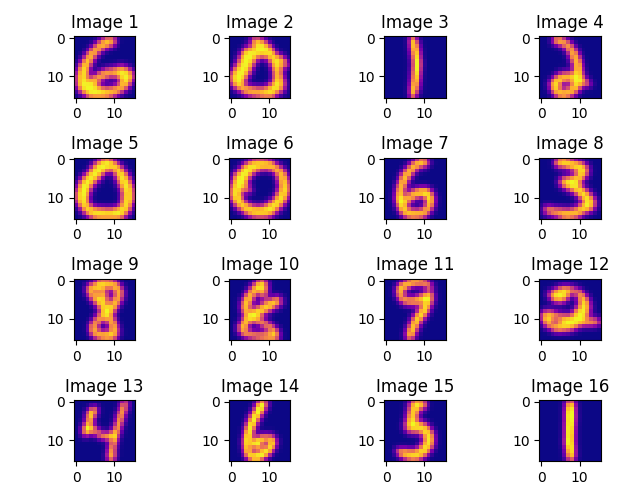
\includegraphics[width = 0.75\textwidth]{FPPFigure_1.png}
	\caption{First 16 train pattern images}
	\label{fig: FIG 01}
\end{figure}


      \vspace{06pt}

In Figure 01 we display the first 16 columns of the training data set. By taking each column and reshaping it to a 16x16 plot each value form [-1, 1] corresponds to a color on the gradient. We are able to see rough images of the digits.

  \section{THE CENTROID CLASSIFICATION ALGORITHM}
    \label{SECT 03:THE CENTROID ALGORITHM}

      \vspace{06pt}
This is a very simple algorithm. Given that each digit, regardless of handwriting style, has the same basic form, we can assume the pattern values (the length 256 column) for a digit $k$ is similar to another image in the set that is labeled as the same digit. We can find the averages of each of these values to determine “the average pattern” for each digit. Then we can compare these averages to the images in our training set and the training average that is the most similar is the chosen predicted digit.  However, if there was great variation in the patterns for each digit, such as very different or messy handwriting, this classification method would have trouble creating clear average patterns.
      
      \subsection{DESCRIPTION OF THE ALGORITHM}
        \label{SUBSECT 3.1:CENTROID DESCRIPTION}

The algorithm: Let $k \in [1,10]$. This means our target digit is $k-1$. We select all column indices in the train labels set where the $k$th row is equal to 1. Use the selected column indices to subset the train patterns and find the row means. This yields a length 256 vector. Repeat for all $k$ to create a $256\times10$ dataset containing the average image patterns for each digit.

        
          \vspace{06pt}


                  \begin{figure}[h!]
	\centering
	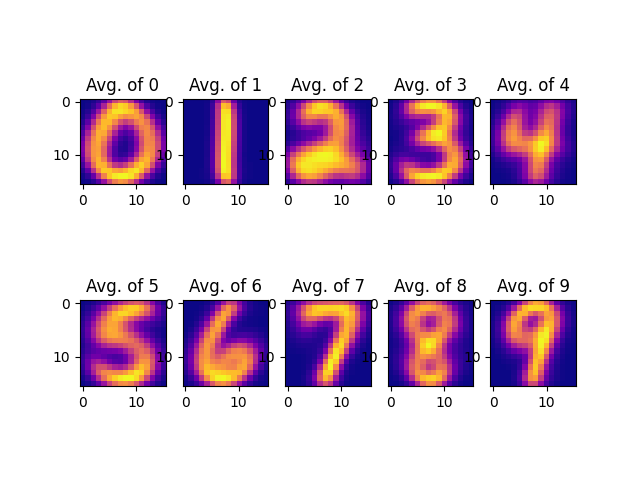
\includegraphics[width = \textwidth]{FPPFigure_2.png}
	\caption{10 mean digit images}
	\label{fig: FIG 02}
\end{figure}


          \vspace{06pt}
          
In Figure 02 we display each of the vectors in the train averages set. This is the average image, or centroid, for each digit.

          \newpage

      \subsection{DESCRIPTION OF THE RESULTS}
       \label{SUBSECT 3.2:CENTROID RESULTS}


\vspace{06pt}
   
                  \begin{figure}[h!]
	\centering
	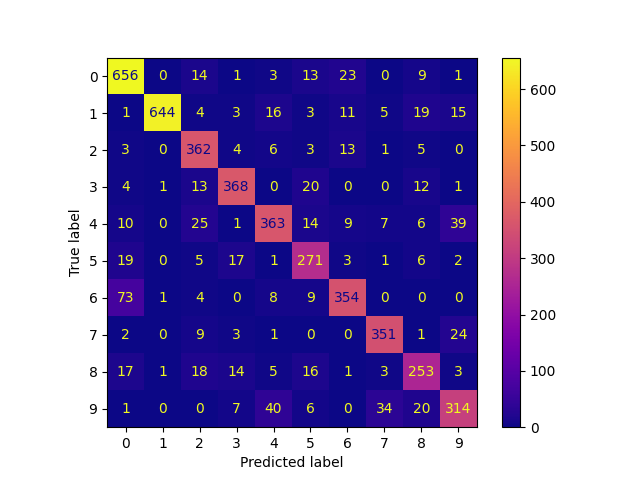
\includegraphics[width = \textwidth]{FPPtest_confusion.png}
	\caption{Confusion matrix of Centroid Algorithm Results}
	\label{fig: FIG 03}
\end{figure}

          \vspace{06pt}
          
          The confusion matrix shows the predicted values on the x-axis, against the test values on the y-axis. There are $n=10$ target classes (the digits) which are labeled on the axes. The values in each box represents the count for each situation on the table. The values correspond to a gradient to enhance readability.
          
          \vspace{06pt}
          
          The rows correspond to the actual or expected label, and the columns correspond to the predicted labels. The diagonal entries are the correctly predicted values. This can be understood intuitively since if the expected value is equal to the predicted value then it falls on $x=y$ or the diagonal. 


      \section{THE SVD CLASSIFICATION ALGORITHM}
        \label{SECT 04:SVD CLASSIFICATION ALGORITHM}

        \vspace{06pt}

The Singular Value Decomposition (SVD) is a powerful matrix factorization method that decomposes a matrix into 3 smaller matrices, the left singular vectors $U$, a diagonal matrix of the singular values $\Sigma$, and the right singular vectors $V^T$. 

        \vspace{06pt}

In this use case,  we do rank reduction by setting the rank = 17  in order to only use the 17 largest singular values to save computation time and space while still retaining the most important information from the original matrix. We use the left singular values or $U$ matrix in order to calculate the expansion coefficients.


        \subsection{DESCRIPTION OF THE ALGORITHM}
          \label{SECT 04.01:SVD DESCRIPTION}

          \vspace{06pt}

          We want to compute SVD for each $k$ value. In this case we are only interested in the left singular vectors, or matrix $U$. When we compute SVD at rank 17, $U$ has the dimensions $256\times17$. Since we calculate this for all values of $k$, we get a three dimensional matrix of size $256\times17\times10$.

     \vspace{06pt}
     
     Next, we want to calculate the expansion coefficients or pattern predictions coefficients based on the SVD basis and test pattern set. The expansion coefficients for a digit $k$ is defined by $U_k^TA$, where $A$ is the test pattern set. Since $U_k^T$ has dimension $17\times256$ and the test pattern set has dimensions $256\times4649$, for each $k$ we get a $17\times4649$ matrix. This yields another 3D matrix of expansion coefficients for each image and each digit of size $17\times4649\times10$.



        \subsection{DESCRIPTION OF THE RESULTS}
          \label{SECT 04.02:SVD RESULTS}
          
          \vspace{06pt}
          
          Finally, we compute the error between the test digit image and the rank 17 approximation. To find the rank 17 approximation or prediction is found by $U_k(U_k^TA)$ where $A$ is the test pattern set. In other words, it is the product of the left singular vectors of a given $k$ and the expansion coefficients found in Section 4.1(b). This provides an approximation using the SVD basis for each image and digit, yielding a $256\times4649\times10$ matrix. We choose to compute the error by calculating the 2-norm between the points because it provides a value of Euclidean distance between the vectors, minimizing this distance allows us to determine the best fit. To calculate these distances we want to select each image $i$ and the $k$ approximations, calculating and recording the 2-norm between each of those 10 vectors and the $i$th column of the test pattern. In theory, the row index of the minimum error, or 2-norm, in each column will provide the correct classification of the digit.
      
   %         \pdfbookmark[2]{Step~05~(c)}{Step_05_(c)}

   %          \pdfbookmark[2]{Step~05~(d)}{Step_05_(d)}

            \newpage

          \begin{figure}[h!]
	\centering
	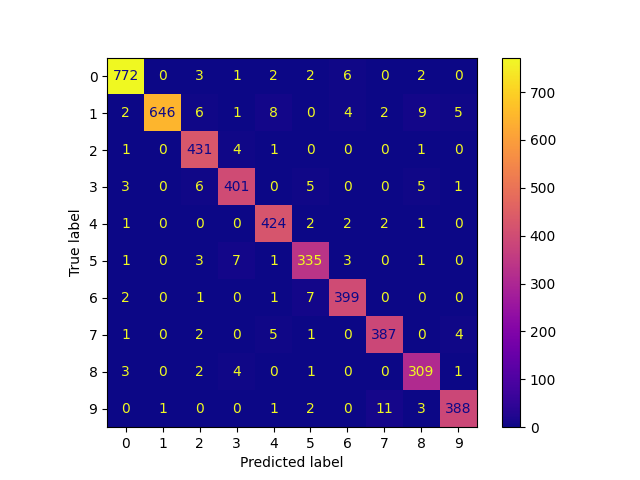
\includegraphics[width = \textwidth]{FPPtest_svd17_confusion.png}
	\caption{Confusion Matrix of SVD Algorithm Results}
	\label{fig: FIG 04}
\end{figure}

\vspace{06pt}

This confusion matrix shows that the SVD algorithm has a very successful performance on this problem. If we sum the values across the diagonal (the correctly predicted values) and divide it by the total number of samples (4649) we can determine the accuracy. The accuracy in this case is $4492/4649 \approx 96.62\%$. This algorithm is almost 100\% accurate.

      \section{ANALYSIS}
        \label{SECT 05:ANALYSIS}


        \vspace{06pt}
        
        In total the Centroid Algorithm had an accuracy of $3936/4649 \approx 84.66\%$. For each digit [0,9], the classification rate is shown in the table below.  

\newpage
              
 \begin{table}[]
\begin{tabular}{|l|l|l|l|l|l|l|l|l|l|l|}
\hline
         & 0      & 1      & 2      & 3      & 4      & 5      & 6      & 7      & 8      & 9      \\ \hline
Centroid & 0.9111 & 0.9411 & 0.9118 & 0.7763 & 0.7658 & 0.8338 & 0.7884 & 0.8909 & 0.7643 & 0.7441 \\ \hline
SVD      & 0.9783 & 0.9458 & 0.984  & 0.9525 & 0.9815 & 0.9544 & 0.9756 & 0.9675 & 0.9656 & 0.9557 \\ \hline
\end{tabular}
\end{table}

    \vspace{06pt}
    
    We can see that the SVD algorithm performed better for every digit when compared to the Centroid algorithm. The Centroid Algorithm was best at recognizing ones. This is most likely due to the unique shape of a 1 as a single vertical line which is distinct from the other digits. The most difficult digit for this algorithm to identify was nines. Its classification was most often confused with the digit 4. This makes sense since they both have a vertical stem and a section at the top that can be enclosed on a 4. When looking at the average digit images of 4 and 9 in Figure 2, we see that the image for 4 is quite blurry, making it difficult for the algorithm to properly differentiate from 9.
    
    \vspace{06pt}

The SVD algorithm was best at identifying the digit 2. This makes sense when taking into account the SVDs algorithm’s ability to represent complex patterns through rank reduction. The approximations were most likely able to better capture the unique shape of a 2 as well as the different ways people draw a 2 (i.e. with a curved tail, with a loop).  The SVD algorithm struggled the most with the digit 1. This is most likely due to the fact that many of the other digits contain a vertical line such as 4 and 9, so it would sometimes misinterpret the complexity of the number. Also, some people write there ones with small horizontal tails at the tops and/or bottoms so that can also play a role in the confusion. 

\vspace{06pt}

The SVD algorithm requires a lot more computation than the Centroid algorithm and thus is slower. It also requires more storage as there are multiple 3D arrays that are produced. Although these are both cons of the SVD algorithm, it is undeniably more accurate than the Centroid algorithm. The classification rate is over 10\% greater than the Centroid algorithm. The SVD algorithm is better at handling more complex images since it accounts for more variability; however the centroid algorithm’s strong suit is simpler, more distinct images. The Centroid algorithm is faster and requires much less storage. It is difficult to determine how to define or quantify better. It depends on the use case which is more optimal. I would argue that for a case where the classifications just need to be generally accurate and there is human supervision to adjust small errors, the Centroid algorithm is adequate. On the other hand, the SVD algorithm is much more reliable. Potentially I would increase the rank of the SVD algorithm to see if that increases the accuracy. If so, that would lead to $\leq 0.01$ misclassification rate which would be consistently reliable for providing accurate results. In that case, the computation and storage would increase by a small amount but it is a trade for near perfect accuracy. In situations where accuracy is the top objective, the SVD algorithm is favored. 

    \vspace*{12pt}

  \section{CONCLUSIONS}
    \label{SECT 06:CONCLUSIONS}

    \vspace{06pt}
A pattern recognition classification algorithm is typically used by mail systems like USPS to read zip codes on envelopes. We create our own digit recognition algorithm by using two classification methods: Centroid algorithm and Singular Value Decomposition (SVD) algorithm.
\vspace{06pt}

There are 9298 samples each containing 256 pixels information of an image of a single digit. This data is split into training data and test data, each with 4649 images. We used the training data to develop our algorithm and used the test set to evaluate the performance.

\vspace{06pt}

In the Centroid Algorithm we collected mean pixel values for each $k$ digits. We then compared each of these averages to the test patterns and chose the digit vector that minimized Euclidean distance as the best fit. 

\vspace{06pt}

In the SVD algorithm we used the largest 17 left singular vectors in order to find expansion coefficients and fit them in the SVD basis. Similar to the previous algorithm, we chose the digit whose corresponding SVD vector minimized the Euclidean distance, or 2-norm, to the test pattern. 

\vspace{06pt}

Through these computations we found that the SVD algorithm is much more accurate than the Centroid algorithm however both algorithms have their strengths and weaknesses. In cases where generalizations are required and efficiency is prioritized, the centroid algorithm is optimal. In cases where accuracy is favored and efficiency is not as important, the SVD algorithm is a better fit.
    
\vspace{06pt}

Different algorithms are required in different cases. The Centroid algorithm and the SVD algorithm are only two of many ways that pattern recognition is done. This exercise provides a glimpse into how pattern recognition automation is developed in industry.


\end{document}
